% !TEX TS-program = pdflatex
% !TEX encoding = UTF-8 Unicode

% This is a simple template for a LaTeX document using the "article" class.
% See "book", "report", "letter" for other types of document.

\documentclass[12pt]{article} % use larger type; default would be 10pt
\usepackage[utf8]{inputenc}   % set input encoding (not needed with XeLaTeX)

%%% PAGE DIMENSIONS
\usepackage{geometry}
\geometry{a4paper}
\geometry{margin=1in} % 1in page margin

%%% COLOR AND GRAPHICS
\usepackage{color}
\usepackage{graphicx} % support the \includegraphics command and options

\usepackage{pslatex}
\definecolor{mygreen}{rgb}{0,0.6,0}
\definecolor{mygray}{rgb}{0.5,0.5,0.5}
\definecolor{mymauve}{rgb}{0.58,0,0.82}
\usepackage{listings} % For displaying source code
\lstset{ %
  language=C,                      % the language of the code
  backgroundcolor=\color{white},   % choose the background color; you must add \usepackage{color} or \usepackage{xcolor}
  basicstyle=\sffamily\fontsize{11}{13.2}\selectfont,        % the size of the fonts that are used for the code
  breakatwhitespace=false,         % sets if automatic breaks should only happen at whitespace
  breaklines=true,                 % sets automatic line breaking
  captionpos=t,                    % sets the caption-position to bottom
  commentstyle=\color{mygreen},    % comment style
  deletekeywords={...},            % if you want to delete keywords from the given language
  escapeinside={\%*}{*)},          % if you want to add LaTeX within your code
  extendedchars=true,              % lets you use non-ASCII characters; for 8-bits encodings only, does not work with UTF-8
  frame=single,                    % adds a frame around the code
  keepspaces=true,                 % keeps spaces in text, useful for keeping indentation of code (possibly needs columns=flexible)
  keywordstyle=\color{blue},       % keyword style
  morekeywords={*,...},            % if you want to add more keywords to the set
  numbers=left,                    % where to put the line-numbers; possible values are (none, left, right)
  numbersep=5pt,                   % how far the line-numbers are from the code
  numberstyle=\color{mygray},      % the style that is used for the line-numbers
  rulecolor=\color{black},         % if not set, the frame-color may be changed on line-breaks within not-black text (e.g. comments (green here))
  showspaces=false,                % show spaces everywhere adding particular underscores; it overrides 'showstringspaces'
  showstringspaces=false,          % underline spaces within strings only
  showtabs=false,                  % show tabs within strings adding particular underscores
  stepnumber=1,                    % the step between two line-numbers. If it's 1, each line will be numbered
  stringstyle=\color{mymauve},     % string literal style
  tabsize=2,                       % sets default tabsize to 2 spaces
  title=\lstname                   % show the filename of files included with \lstinputlisting; also try caption instead of title
}

% \usepackage[parfill]{parskip} % Activate to begin paragraphs with an empty line rather than an indent

%%% PACKAGES
\usepackage{booktabs} % for much better looking tables
\usepackage{array}    % for better arrays (eg matrices) in maths
\usepackage{paralist} % very flexible & customisable lists (eg. enumerate/itemize, etc.)
\usepackage{verbatim} % adds environment for commenting out blocks of text & for better verbatim
\usepackage{subfig}   % make it possible to include more than one captioned figure/table in a single float

%%% HEADERS & FOOTERS
%\usepackage{fancyhdr} % This should be set AFTER setting up the page geometry
%\pagestyle{fancy} % options: empty , plain , fancy
%\renewcommand{\headrulewidth}{0pt} % customise the layout...
%\lhead{}\chead{}\rhead{}
%\lfoot{}\cfoot{\thepage}\rfoot{}


%%% SECTION TITLE APPEARANCE
\usepackage{sectsty}
\sectionfont{\normalsize\bfseries\uppercase}
\subsectionfont{\normalsize\bfseries}
\subsubsectionfont{\normalsize\mdseries\itshape}

%%% ToC (table of contents) APPEARANCE
\usepackage[nottoc,notlof,notlot]{tocbibind} % Put the bibliography in the ToC
\usepackage[titles,subfigure]{tocloft} % Alter the style of the Table of Contents
\renewcommand{\cftsecfont}{\rmfamily\mdseries\upshape}
\renewcommand{\cftsecpagefont}{\rmfamily\mdseries\upshape} % No bold!

%%% Title setup
\newcommand{\TitleFont}{\fontsize{16}{20}\selectfont\bfseries}
\newcommand{\AuthorFont}{\fontsize{14}{17}\selectfont}

%%% END Article customizations

%%% The "real" document content comes below...

\title{\TitleFont EE 472 Lab 1 \\ Introducing the Lab Environment \vfill }
\author{\AuthorFont Jonathan Ellington \\ Patrick Ma \\ Jarrett Gaddy}
\date{}

\begin{document}

%% Make title and ToC, start page numbering AFTER ToC
\maketitle
\thispagestyle{empty}
\pagebreak
\tableofcontents
\listoftables
\listoffigures
\thispagestyle{empty}
\pagebreak
\setcounter{page}{1}

\section{Abstract}
The abstract should provide a brief overview of the report.  It should provide a summary of the main specific points for the introduction, the main tests and experiments, the results, and the conclusions. It is called an abstract because you can literally "abstract" sentences from the other sections. 

Once again, this is not a narrative of your experiences as you executed the design.  The abstract should mirror (albeit in a very condensed way) the content of your report.

\section{Introduction}
Brief introduction and overview of the purpose of the lab and of the methods and tools used.

\section{Discussion of the Lab}

This section should include the following:

\subsection{Design Specification}

In this subsection you will textually describe your client's requirements.  What does he or she need in the project you are developing.  If you are incorporating extra features or capabilities, please describe them clearly in this section.

\begin{itemize}[$$]
  \item Overall summary description of the module - 2-3 paragraphs maximum

    \begin{itemize}[$$]
      \item Specification of the public interface to the module

        \begin{itemize}[$\bullet$]
          \item Inputs
          \item Outputs
          \item Side effects
        \end{itemize}

      \item Psuedo English description of algorithms, functions, or procedures
      \item Timing constraints
      \item Error handling
    \end{itemize}
\end{itemize}

\begin{table}[h]
    \centering
    \label{table:ex}
    \begin{tabular}{llr}
        \toprule
        Animal    & Description & Price (\$) \\
        \midrule
        Gnat      & per gram    & 13.65      \\
                  & each        & 0.01       \\
        Gnu       & stuffed     & 92.50      \\
        Emu       & stuffed     & 33.33      \\
        Armadillo & frozen      & 8.99       \\
        \bottomrule
    \end{tabular}
    \caption{Example table.}
\end{table}

\subsection{Software Implementation}

What is your design????

Present your design starting from a top level functional view and potentially block diagram or high level architecture.  Refine that view to present and explain each of the modules that comprise the major functional blocks.  Discuss the flow of control through the design.  Identify and discuss the specific processes/tasks you have implemented in your design. Explain your design choices.    

\begin{figure}[h]
    \centering
    \label{figure:chick}
    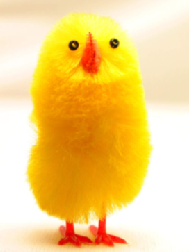
\includegraphics{figure1.png}
    \caption{A chick}
\end{figure}

\section{Presentation, Discussion, and Analysis of the Results}

Based upon the execution of your design, present your results. Explain them and what was expected, and draw any conclusions (for example, did this prove your design worked).

In addition to a detailed discussion and analysis of your project and your results, you must include all the answers to all questions raised in the lab.

\subsection{Analysis of any Errors}

This one is obvious. Do this section as appropriate.  If it improves the flow, it does not need to be a separate section and may be included in the presentation, discussion, and analysis of the results.  However, it will still be graded separately and must be present.

\subsection{Analysis of why the project may not have worked and what efforts were made to identify the root cause of any problems}

State any problems you encountered while working on the project. If your project did not work or worked only partially, provide an analysis of why and what efforts were made to identify the root cause of any problems.

\section{Test Plan}

Overall summary of what needs to be tested to ensure that your design meets the original requirements, 2-3 paragraphs maximum unless specified otherwise

\subsection{Test Specification}

Annotated description of what is to be tested and the test limits.  This specification quantifies inputs, outputs, and constraints on the system.  That is, it provides specific values for each. 

Note, this does not specify test implementation...this is what to do, not how to do it.

\subsection{Test Cases}

Annotated description of how your system is to be tested against the test limits
Note, this does specify test implementation...this is not what to do, this is how to do it based upon the test specification.

\section{Summary and Conclusion}

You should know these sections very well, no need to explain.  Note, however, that they are two different sections.  The summary is just that, a summary of your project.  It should loosely mirror the abstract with a bit more detail.  The conclusion concludes the report, potentially adds information that is often outside the main thrust of the report, and may offer suggestions or recommendations about the project.

\pagebreak
\appendix

\section{Source Code}
\subsection{The first part}
\lstinputlisting{source.c}

\subsection{The second part}
\lstinputlisting{source.c}

\end{document}
